\section{实验}
\label{sec:experiments}

\subsection{范围与评测协议}

任务是3D--3D配准，残差为
$\mathbf{r}_i=R(\mathbf{q})\mathbf{p}_i+\mathbf{t}-\mathbf{y}_i$，除另述外使用$c=0.05$~m的GM核，
成功定义为旋转误差$<5^\circ$且平移误差$<0.1$~m。RANSAC使用3点采样与阈值$\|\mathbf{r}_i\|<c$；
\emph{固定}基线总是花费1000次迭代（v0协议），\emph{自适应}基线使用标准的0.999置信界并截断于
1000。除非另述，每个单元格50--100次试验并使用固定种子；运行时间为共享CPU节点上单次调用的墙钟
p50/p95，故加速比是同一次运行内的比值。对100、160、60、40次试验的单元格，Wilson $95\%$下界分别为
$96.3\%$、$97.7\%$、$94.0\%$、$91.2\%$，因此“$100\%$”并非精确速率。前向求解器是加权Kabsch，
即QPEP的闭式标量权重3D--3D特化；它隔离的是鲁棒估计器与反向，完整的QPEP代数由附录~\ref{app:systems}
中的$4\times4$ Davenport/Horn变体承担。

真实数据评测覆盖全部八个官方3DMatch测试场景（含低/中/高重叠研究与更严格的$0.20$--$0.50$带）、
两次KITTI raw驾驶、全部11个KITTI odometry序列00--10（每个33个选定帧），以及四次UTIAS
In-The-Dark运行：两次各15对的白天运行与两个各10对的夜间窗口，均使用手写SIFT+StereoSGBM前端。

\subsection{合成前向鲁棒性与代价}

\begin{table}[t]
\caption{合成3D--3D在\emph{随机}外点下的成功率（\%），$N=100$，每格100次试验。固定RANSAC
$=1000$次迭代；自适应$=0.999$置信、上限1000。}
\label{tab:synthetic}
\centering
\scriptsize
\setlength{\tabcolsep}{2.2pt}
\begin{tabular}{lccccc}
\toprule
$p$ & Kabsch & RANSAC-1000 & \shortstack{自适应\\RANSAC} & IRLS-GM & GNC-GM \\
\midrule
0\%  & 100 & 100 & 100 & 100 & 100 \\
10\% & 52  & 100 & 100 & 100 & 100 \\
30\% & 0   & 100 & 100 & 100 & 100 \\
50\% & 0   & 100 & 100 & 100 & 100 \\
70\% & 0   & 100 & 100 & 98  & 100 \\
\bottomrule
\end{tabular}
\end{table}

表~\ref{tab:synthetic}报告随机外点（观测被替换为$[-2,2]^3$内均匀采样），每格100次试验，
$N=100$。GNC-GM与两种RANSAC变体在$70\%$以内均为$100\%$；IRLS在$70\%$时降至$98\%$；非鲁棒
Kabsch在$10\%$之后崩溃。所有鲁棒方法的中位旋转误差为$0.13$--$0.21^\circ$；$p=30\%$时
RANSAC-1000为$0.13^\circ$、GNC为$0.14^\circ$，保留两位小数时持平。有意义的差别在代价：GNC p50
为$1.48$--$1.63$~ms，RANSAC-1000为$47.7$--$51.9$~ms，自适应RANSAC为$0.41$--$12.36$~ms。相对
固定的v0基线，GNC在$p\ge10\%$时快$\mathbf{31.6}$--$\mathbf{32.5\times}$；相对自适应RANSAC，
它在低$p$时更慢（$10\%$时$3.9\times$），$40\%$时持平（$1.0\times$），$70\%$时快$8.3\times$
（$80$--$90\%$时快$25$--$30\times$，此时自适应RANSAC到达上限）。RANSAC不可微；GNC的反向是
一次$6\times6$求解。更强的LO-RANSAC（MSAC评分，最多五轮局部重拟合/重评分，0.999自适应停止，
上限1000）在精度上与GNC持平（中位旋转差$\le0.006^\circ$），但本身比普通自适应RANSAC慢
$1.03$--$1.52\times$（附录~\ref{app:ablations}）。由于固定1000预算不是最强的运行时间基线，
下文的每个加速比都注明所比较的预算：GNC比固定1000 RANSAC快$22$--$32\times$，且在高外点率下
运行时间平坦；相对自适应RANSAC，它在低外点比例更慢，$40\%$附近持平，$70\%$时约快$8\times$。

随机外点会美化所有方法。更细的崩溃扫描（每格100--200次试验）显示RANSAC在$80$--$90\%$处失效：
$90\%$随机外点时RANSAC-1000为$51\%$，GNC为$62\%$，IRLS为$32\%$；$80\%$时GNC为$89\%$，而
RANSAC为$100\%$。在存在一个相干竞争刚体变换时，所有方法在$45\%$以内为$100\%$，随后崩溃：
$50\%$时GNC为$52\%$、RANSAC为$50\%$，$55\%$时GNC为$2.5\%$、RANSAC为$0\%$，$60\%$时所有方法
都返回\emph{外点}变换（外点恢复率$100\%$）。这是第~\ref{sec:discussion}节分析的可辨识性失效。
在边界外点（$e/c^2\sim U(1/3,3)$）下，即使$70\%$，所有方法仍为$100\%$，且鲁棒方法更准
（$70\%$时GNC $0.27^\circ$ vs RANSAC $0.62^\circ$与Kabsch $0.33^\circ$）；边界外点的影响主要在
精度而非前向成功率。

\subsection{精确梯度与冻结权重}
\label{sec:gradient}

6D梯度表使用$N=30$，十个$40\%$边界实例与十个$20\%$随机实例，GNC加Newton精化到
$\|\Phi\|\sim10^{-13}$，并对精化后的不动点分支做中心有限差分（$h=10^{-5}$）。精确IFT Jacobian
与FD的相对Frobenius误差为$\mathbf{4.9\times10^{-8}}$（内点）、$\mathbf{3.1\times10^{-8}}$
（边界）、$1.25\times10^{-4}$（粗大，受FD相消限制），余弦为$1.000000$。朴素的冻结权重Jacobian
相对误差为$0.212$（内点）与$\mathbf{1.07}$（边界），边界余弦为$0.234$（最小$-0.358$）。只省略
$-\lambda_{\mathrm{rob}}$项给出$9.0\times10^{-4}$--$9.8\times10^{-4}$的相对误差，因此曲率修正
是主要的缺失项，而不是约束项。

\begin{table}[t]
\caption{6D Jacobian与精化不动点分支的中心有限差分对比（$N=30$）。除标注min外，相对误差与余弦
均为中位数。$^\ast$受FD相消限制；绝对误差仍小且余弦为$1$。}
\label{tab:gradient}
\centering
\footnotesize
\setlength{\tabcolsep}{2.5pt}
\begin{tabular}{llrccc}
\toprule
分箱 & 方法 & $n$ & 相对误差p50 & 余弦p50 & 最小 \\
\midrule
内点   & 精确 & 414 & $4.9\times10^{-8}$ & 1.000000 & 1.000000 \\
内点   & 朴素 & 414 & $2.12\times10^{-1}$ & 0.985 & 0.791 \\
边界 & 精确 & 122 & $3.1\times10^{-8}$ & 1.000000 & 1.000000 \\
边界 & 朴素 & 122 & $\mathbf{1.07}$ & $\mathbf{0.234}$ & $\mathbf{-0.358}$ \\
粗大    & 精确 & 64  & $1.25\times10^{-4\ast}$ & 1.000000 & 0.9986 \\
粗大    & 朴素 & 64  & $1.16$ & $-0.118$ & $-0.397$ \\
\bottomrule
\end{tabular}
\end{table}

对$e>c^2/3$的观测，映射级径向响应在$\mathbf{100\%}$的边界（$122/122$）与粗大（$64/64$）观测上
使精确与朴素符号相反；在这个良态6D样本中，位姿平移级也有$100\%$翻转。一维陈述是定理
（命题~\ref{prop:signflip}）；6D陈述为数值结果。端到端精化诊断（附录~\ref{app:e2e}）表明，
精确梯度在测试时目标上带来改进，而冻结权重梯度没有。

\subsection{真实几何}

\begin{table*}[t]
\caption{实测真实数据汇总。成功为随机外点下旋转$<5^\circ$且平移$<0.1$~m；加速比为GNC-GM p50
相对\emph{固定1000次}RANSAC p50（自适应RANSAC在正文讨论）。“---”$=$不适用；bnd$=$边界外点。}
\label{tab:real}
\centering
\scriptsize
\setlength{\tabcolsep}{2.2pt}
\begin{tabular}{llcccc}
\toprule
数据集 & 子集 & 成功 & 误差 & 加速/备注 \\
\midrule
3DMatch & 8个官方测试场景，每格20次 & $100\%$ $\le70\%$ & $0.27^\circ$ @$70\%$ bnd &
$27.7\times$；相干$46\%$ vs $3\%$ @$50\%$ \\
KITTI raw & drive 0001/0002（108/77帧），10对 & $100\%$ $\le70\%$ &
$0.07$--$0.09^\circ$ @$70\%$ & $\sim22\times$；bnd RANSAC $0.14$--$0.16^\circ$ \\
KITTI odom. & 00--10，每个33帧 & $99/99/100/100\%$ & $0.067^\circ$ @$70\%$ &
$22.4\times$；seq 08 $80\%$ @$p\le0.3$ \\
In-The-Dark 白天 & 2次运行，每次15对 & $100\%$ @$0.1$~m & $0.078$/$0.092^\circ$ &
$0.020$/$0.010$~m；$79.4/88.5\%$ 内点 \\
In-The-Dark 夜间 & 2个窗口，每个10对 & $100\%$ @$0.1$~m & $0.135$/$0.150^\circ$ &
$0.011$~m；$96.0/97.1\%$ 内点 \\
\bottomrule
\end{tabular}
\end{table*}

\noindent\textbf{ModelNet40/10。}在真实物体点云、每格50次试验与均匀外点下，GNC-GM在两个数据集上
$0$--$70\%$均为$100\%$；RANSAC-1000为$100\%$，IRLS为$98$--$100\%$，Kabsch在$50\%$崩溃。GNC为
$1.7$--$1.9$~ms vs $53.5$--$61.5$~ms（$30$--$32.5\times$）。ModelNet10（908个测试物体、10类、
2048点）与ModelNet40的成功率最多相差$2$个百分点，中位旋转最多相差$0.038^\circ$。

\noindent\textbf{3DMatch。}全部八个官方测试场景都用官方TSDF点云与\texttt{gt.log}处理，采用GT
映射的最近邻对应（具有真实扫描/遮挡残差的oracle匹配），$N=300$，$c=0.05$~m，每格20次试验，
每场景8对高重叠对。随机外点：GNC与RANSAC-1000在$70\%$以内均为$100\%$（IRLS在$70\%$为
$99\%$），汇总GNC p50为$2.26$~ms vs $62.6$~ms（$27.7\times$；逐场景$2.26$--$2.36$ vs
$62.1$--$73.4$~ms，$27.4$--$31.1\times$）。相干外点在$60$--$70\%$时所有方法崩溃（$0\%$）；
$50\%$时GNC为$46\%$、RANSAC为$3\%$。低/中/高重叠研究（24/21/20对）给出的干净旋转为
$0.52/0.24/0.18^\circ$，两种鲁棒方法在每个分箱、$p=0.7$时均为$100\%$（$p\ge30\%$时加速
$27.7$--$30.4\times$）；更严格的$0.20$--$0.50$几何重叠带其oracle基础内点率为$0.953$/$0.984$，
干净旋转$0.47^\circ$/$0.19^\circ$，其中GNC与RANSAC在$p=0.7$时仍为$100\%$（IRLS $92\%$，
Kabsch $1\%$）。一个手工FPFH前端（匹配中不使用GT）达到$80.0\%$/$67.8\%$的自然内点率，GNC为
$100\%$/$100\%$，RANSAC-1000为$100\%$/$97\%$，Kabsch为$100\%$/$83\%$。

\noindent\textbf{KITTI。}两次raw驾驶（2011\_09\_26的drive 0001/0002，108/77帧）给出真实室外
LiDAR，OXTS运动映射到Velodyne。$N=300$，$c=0.25$~m，10对、每格20次试验时，GNC与RANSAC-1000
在$70\%$以内均为$100\%$；GNC p50为$2.7$--$2.8$~ms vs $61$--$64$~ms（$\sim22\times$），相干
$60$--$70\%$时所有方法崩溃，边界情形GNC与IRLS为$100\%$（$70\%$时$0.07$--$0.09^\circ$ vs
RANSAC $0.14$--$0.16^\circ$）。Drive 0002复现了这些表格与相干转变（$50\%$时GNC $40\%$ vs
$35\%$，IRLS $30\%$ vs $45\%$）。对odometry，全部11个序列00--10各由33个选定帧代表；在新增的
八个序列上（每格10次试验），$p=0.7$时GNC与RANSAC-1000均为$100\%$，唯seq~08例外：GNC在$p=0$
和$p=0.3$时为$80\%$（RANSAC为$100\%$）。11个序列汇总的成功率为$p=0/0.3/0.5/0.7$时
$99/99/100/100\%$，$p\ge0.3$时固定RANSAC/GNC运行时间比为$22.4\times$。00/05/07子集补充了
相干崩溃（$p=0.6$；$p=0.5$时GNC $53\%$，IRLS $38\%$，RANSAC $0\%$）、边界$0.067^\circ$ vs
$0.143^\circ$，以及在$|\mathbf{t}|=0.09$--$9.62$~m与间隔$1/2/4/8$的171个配对单元格上GNC
从未低于RANSAC。干净下限$0.042$--$0.057^\circ$并不低于OXTS驱动（$0.030$--$0.039^\circ$），
故主导它的是LiDAR采样。

\noindent\textbf{UTIAS In-The-Dark \cite{utias2020inthedark}。}官方逐对GT由重复空间$\times$示教
时间$\times$相机--车辆共轭复合而成，并用双目重投影验证（中位$0.52$--$0.65$~px，而逆、恒等与
未共轭替代为$9.5$--$31.3$~px）。每次运行的15对连续白天图像、手写SIFT+StereoSGBM前端下，自然
内点率为$79.4\%$/$88.5\%$，GNC-GM达到$\mathbf{0.078^\circ/0.020}$~m与
$\mathbf{0.092^\circ/0.010}$~m，$0.1$~m成功率$100\%$（Kabsch $47\%/40\%$）。两个夜间窗口
（run\_000017/18），各10对连续图像：稠密SGBM给出$96.0\%$/$97.1\%$内点，GNC为
$0.135^\circ/0.011$~m与$0.150^\circ/0.011$~m，$0.1$~m成功率均$100\%$；稀疏夜间为$84.3\%$与
$0.197^\circ/0.015$~m。一个运动匹配的白天对照给出$85.9\%$内点与$0.121^\circ/0.007$~m，故夜间
内点优势主要是更近距/几何效应（夜间中位深度$4.5$~m，白天$6.7$--$7.2$~m）。

\noindent\textbf{KITTI双目前端。}在矫正后的\texttt{image\_02/03}（$b=0.5327$~m）上使用SIFT+
亚像素+StereoSGBM前端，drive 0001的30对给出自然内点率$17.8\%$（$c=0.5$~m），每对890个对应。
GNC/IRLS把旋转恢复到$0.052^\circ$（GT内点下限$0.071^\circ$），但平移中位$0.70$~m vs
$1.92$~m运动与$0.239$~m下限；没有方法达到$0.1$~m或$0.25$~m成功。GNC比固定RANSAC快
$19.3\times$（4.21 vs 81.3~ms）。$3$--$60$~m上双目与LiDAR深度比为$1.000$--$1.061$，排除了
视差尺度误差，故该层修正了旋转但继承了前端的平移偏置。

\begin{figure}[t]
\centering
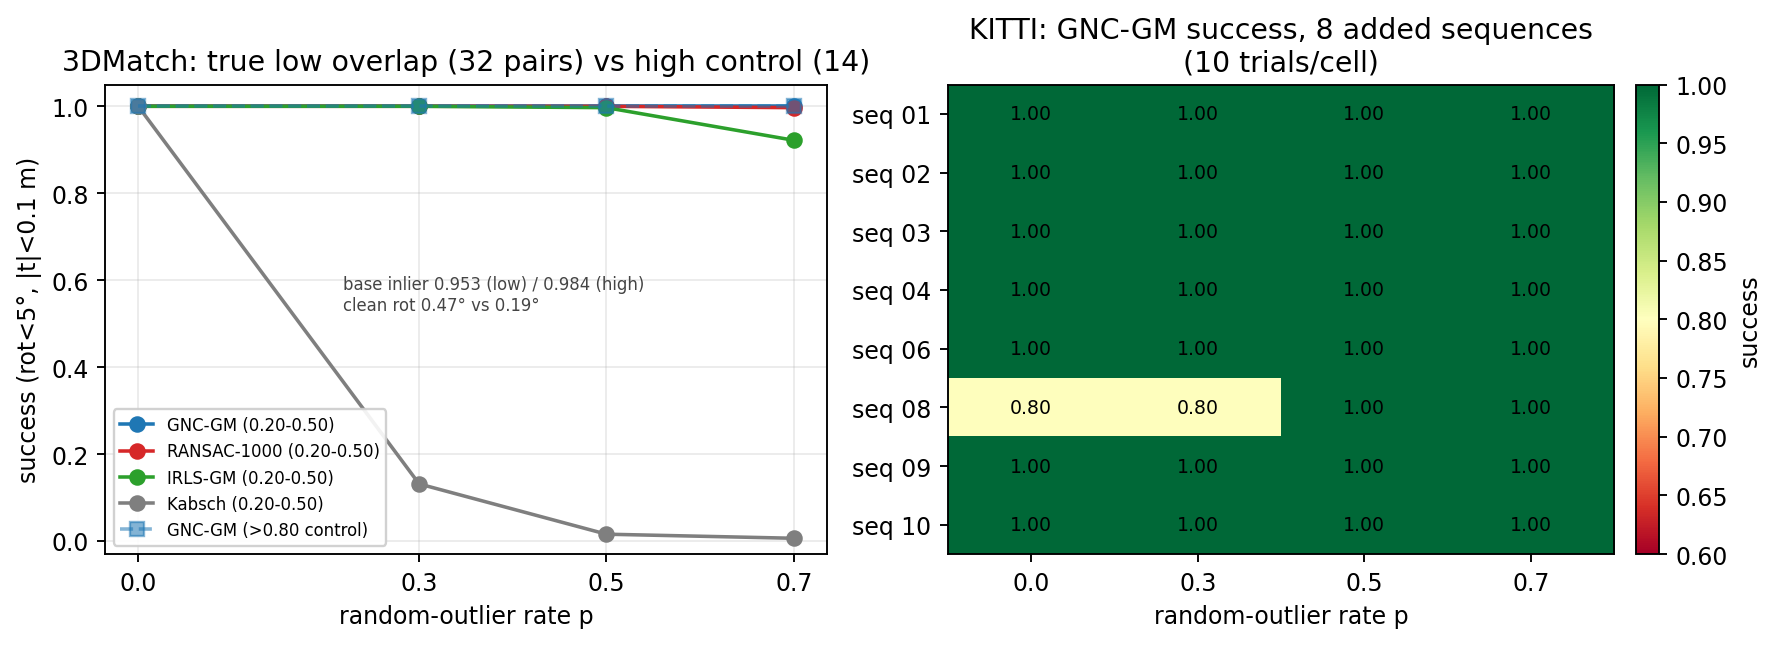
\includegraphics[width=0.75\columnwidth]{p3_data_coverage.png}
\caption{真实数据覆盖。左：3DMatch低重叠（$0.20$--$0.50$，32对）相对高重叠对照（14对），
每格10次试验。右：GNC-GM在新增八个KITTI odometry序列上的成功率；seq~08在$p=0$和$p=0.3$时
为$80\%$。}
\label{fig:coverage}
\end{figure}

\subsection{系统、基线与消融}

一个在$(B,N,3)$上向量化的NumPy GNC把循环复现到$1.1\times10^{-14}$（旋转）与
$1.2\times10^{-15}$（平移）；$B=32,N=100$时批处理p50为$8.5$~ms vs $56.2$~ms（$6.60\times$），
$B=8$给出$2.95\times$/$3.27\times$，$B=1$更慢（$0.54\times$）。$4\times4$的Davenport/Horn
内层求解器\cite{horn1987}在数值上等价于加权Kabsch（最大$\|R_d-R_k\|_F=1.07\times10^{-14}$，
代价超出$9.4\times10^{-16}$），但只在大$N$时更快。在合成数据上，Theseus-GM随机初始化下
$p=0/0.3/0.5/0.7$时为$100/80/55/25\%$，耗时$358$--$670$~ms，而GNC-GM在同一20个实例上以
$1.7$~ms达到$100\%$（$p=0.3$的Wilson区间重叠）；SDPRLayers+SCS数值上可用（$0/208$异常，
$8.5$--$13.4$~ms），但只在$p=0$成功，且$W_i=I$时退化为Kabsch。核、调度、RANSAC强度与
各向异性权重消融见附录~\ref{app:ablations}。
